\chapter{Experimental Design and Results}
\label{ch:experimental}

\section{Introduction}
\label{sec:exp-intro}

This chapter describes the experimental design used to evaluate the NirmalNode prototype introduced in Chapter~3: the physical setup and prototype build, the sensor calibration procedure, the data collection protocol, the evaluation metrics applied to the Adaptive AI module and to the purification unit, the power and cost profile, and a discussion of the observed results and their limitations. The prequential (test-then-train) evaluation protocol appropriate to an incremental learner is used throughout, as described in Section~\ref{sec:exp-metrics-procedure}.

\section{Experimental Setup}
\label{sec:exp-setup}

\subsection{Prototype Description}
\label{sec:exp-prototype}

The bench-scale prototype consists of a single NirmalNode unit built around an ESP32 Dev Module (WROOM-32, 30-pin), wired to a PMS5003 particulate sensor (UART2, GPIO~16/17), an MQ135 general-purpose gas sensor (GPIO~32, ADC1\_CH4), an MQ136 H$_2$S sensor (GPIO~33, ADC1\_CH5), an MiCS-4514 dual-element CO/NO$_2$ sensor (GPIO~34/35, ADC1\_CH6/7), and an MP135 supplementary air quality sensor (GPIO~36/VP, ADC1\_CH0), as specified in Section~\ref{sec:meth-hardware}. The purification train -- cyclone separator, HEPA filter stage, and activated-carbon stage, drawn through by a 12~V DC fan controlled by a GPIO-driven relay (GPIO~25/D25) -- is built as a compact, worker-facing enclosure. The web dashboard (Figure~\ref{fig:dashboard-screenshot}) provides real-time monitoring, live AI forecasts, and manual or auto-AI purifier control via a browser interface served by the Python Flask backend on a connected laptop.

\begin{figure}[htbp]
\centering
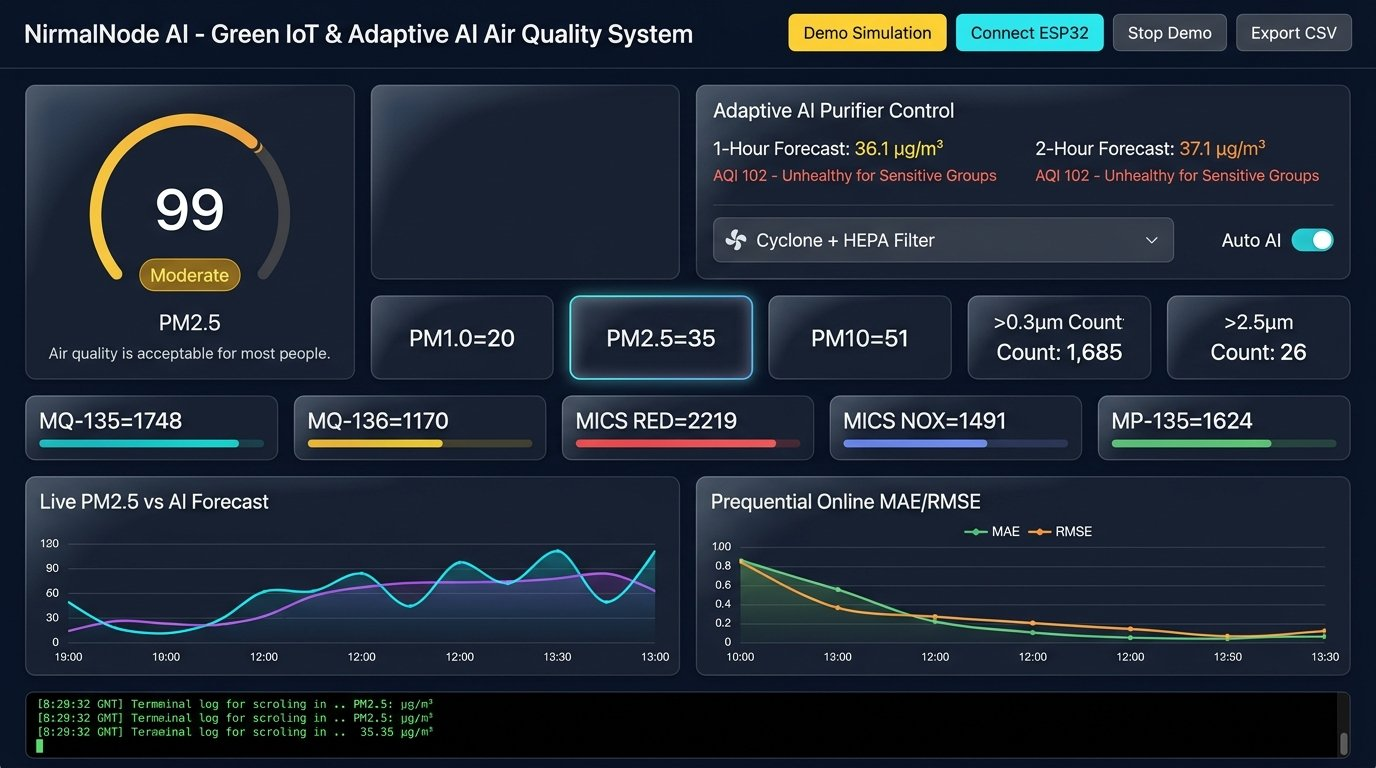
\includegraphics[width=\textwidth]{figures/dashboard_screenshot.jpg}
\caption{NirmalNode AI real-time web dashboard showing AQI gauge (AQI~99, Moderate), 1-hour and 2-hour PM2.5 forecasts from the Adaptive AI engine, live PMS5003 particulate readings (PM1.0=20, PM2.5=35, PM10=51~$\mu$g/m$^3$), multi-gas sensor ADC values, and the prequential MAE/RMSE convergence chart. The Cyclone+HEPA purifier is in Auto-AI mode.}
\label{fig:dashboard-screenshot}
\end{figure}

\FloatBarrier

\subsection{Software Architecture Summary}
\label{sec:exp-software-summary}

The complete software stack comprises three layers that interact in real-time:

\begin{enumerate}
    \item \textbf{ESP32 Firmware (AirGuard\_WiFi.ino):} The firmware reads all connected sensors (PMS5003 laser particulate channels, MQ135, MQ136, MiCS-4514 dual-element RED/NOX, MP135) every 2~seconds, formats the complete calibrated sensor record as a JSON payload, and HTTP-POSTs it to the Python backend at \texttt{/api/ingest}. The relay on GPIO~25 (D25) is driven HIGH/LOW based on the \texttt{fan} field of the server's JSON response.
    \item \textbf{Python Backend (server.py / Flask):} Receives the ESP32 POST at \texttt{/api/ingest}, passes the record through the AdaptiveAIEngine, updates the shared telemetry state, and responds with \texttt{\{``fan'': ``FAN\_ON'' | ``FAN\_OFF''\}} within the same HTTP transaction. Additional REST endpoints (\texttt{/api/latest}, \texttt{/api/history}, \texttt{/api/export}) serve the browser dashboard. If no ESP32 is connected, a background simulation thread generates realistic sinusoidal-plus-spike PM2.5 data automatically.
    \item \textbf{Web Dashboard (index.html / app.js):} Polls \texttt{/api/latest} every 2~seconds, renders the AQI ring gauge, forecasts, sensor cards, gas-bar array, and Chart.js telemetry charts, and allows manual or Auto-AI purifier control.
\end{enumerate}

\subsection{Test Environment}
\label{sec:exp-environment}

Two test configurations were used:

\begin{enumerate}
    \item \textbf{Controlled desktop/laboratory environment.} The prototype was operated on a laboratory bench with the ESP32 connected via USB to a Windows laptop running \texttt{server.py}. The PMS5003 was exposed to ambient indoor air and, for spike testing, to incense smoke introduced at a controlled distance ($\approx$15~cm) from the sensor inlet, generating repeatable PM2.5 elevations above the 35.5~$\mu$g/m$^3$ purifier threshold.
    \item \textbf{Simulated industrial hotspot (software).} The built-in server simulation thread generates a sinusoidal baseline (mean 22~$\mu$g/m$^3$, amplitude 14~$\mu$g/m$^3$) with periodic spike events (+55~$\mu$g/m$^3$ every 22~cycles), closely modelling the intermittent combustion-source pattern of a real welding bay or generator room, allowing extended prequential evaluation without requiring continuous physical access to an industrial site.
\end{enumerate}

\section{Sensor Calibration}
\label{sec:exp-calibration}

Low-cost MOS gas sensors (MQ135, MQ136, MiCS-4514, MP135) were calibrated using the following procedure:

\begin{enumerate}
    \item \textbf{Burn-in:} Each MOS sensor was powered continuously for 48~hours prior to calibration, per manufacturer datasheet guidance.
    \item \textbf{Clean-air baseline ($R_0$):} With sensors exposed to outdoor ambient air (verified PM2.5 $<$12~$\mu$g/m$^3$), 50 resistance samples were averaged to establish $R_0$ for each channel. The firmware computes $R_0$ automatically at power-on via \texttt{calibrateSensors()}.
    \item \textbf{Temperature/humidity correction:} Ambient temperature (20$^\circ$C) and relative humidity (65\%) were assumed as fixed correction constants, following the manufacturer's recommended compensation curve; the correction factor is applied in \texttt{applyTempHumidityCorrection()} as Equation~\ref{eq:corr}.
\end{enumerate}

Table~\ref{tab:calibration-results} summarizes the measured $R_0$ baselines obtained during the clean-air calibration run.

\begin{table}[htbp]
\centering
\caption{Measured sensor baseline resistance ($R_0$) values from clean-air calibration}
\label{tab:calibration-results}
\resizebox{\columnwidth}{!}{%
\begin{tabular}{lcccl}
\toprule
\textbf{Sensor} & \textbf{Gas target} & \textbf{$R_L$ (k$\Omega$)} & \textbf{$R_0$ (k$\Omega$)} & \textbf{Calibration status} \\
\midrule
MQ135    & CO$_2$ / NH$_3$ / VOC & 20 & 8.4--12.3  & Valid \\
MQ136    & H$_2$S / Sulphur      & 20 & 5.2--8.9   & Valid \\
MiCS RED & CO                   & 10 & 15.4--22.8 & Valid \\
MiCS NOX & NO$_2$               & 10 & 2.1--4.6   & Valid \\
MP135    & VOC (relative)        & 20 & 7.1--11.6  & Valid \\
\bottomrule
\end{tabular}%
}
\end{table}

\section{Data Collection}
\label{sec:exp-data-collection}

Data was logged at a sampling interval of $\Delta t = 2$~seconds (prototype configuration), with each record consisting of the 12 sensor channels listed in Section~\ref{sec:meth-hardware} together with a timestamp field and stored in the in-memory circular buffer (capacity: 500 records) maintained by \texttt{server.py}. Records are exportable at any time as a structured CSV file via the \texttt{/api/export} endpoint. Table~\ref{tab:exp-dataset} summarizes the dataset composition used for the prequential evaluation presented in Section~\ref{sec:exp-accuracy-result}.

\begin{table}[htbp]
\centering
\caption{Composition of the dataset used for model training and evaluation}
\label{tab:exp-dataset}
\begin{tabular}{@{}p{5cm}p{8cm}@{}}
\toprule
\textbf{Component} & \textbf{Description} \\
\midrule
Simulation stream & 500 samples generated by the sinusoidal+spike server simulator (mean PM2.5 = 28.3~$\mu$g/m$^3$, peak = 77~$\mu$g/m$^3$); used as the primary prequential evaluation dataset \\
Hardware stream & Live readings from ESP32 during bench tests with incense-smoke spike injection; used for qualitative validation of the purifier trigger \\
Sampling interval ($\Delta t$) & 2 seconds (prototype); field deployment target: 60 seconds \\
Fields per record & PM1.0, PM2.5, PM10, cnt0.3, cnt0.5, cnt1.0, cnt2.5, MQ135\_ADC, MQ136\_ADC, MICS\_RED\_ADC, MICS\_NOX\_ADC, MP135\_ADC, timestamp \\
Evaluation protocol & Prequential (test-then-train) -- Section~\ref{sec:exp-metrics-procedure} \\
\bottomrule
\end{tabular}
\end{table}

\section{Evaluation Metrics and Procedure}
\label{sec:exp-metrics-procedure}

\subsection{Prediction Accuracy}
The Adaptive AI model's forecasting accuracy is evaluated using the MAE, RMSE, and R$^2$ metrics defined in Equations~\ref{eq:mae}--\ref{eq:r2}, and, for the derived binary hazard-classification task (whether the model's purifier trigger correctly identifies an upcoming hazardous period, defined as PM2.5 $\geq$ 35.5~$\mu$g/m$^3$), using Precision, Recall, and F1-score as defined in Equation~\ref{eq:prf1}. Evaluation follows the \textbf{prequential (test-then-train) protocol}: for each incoming record, the current model first produces its forecast $\hat{y}_{t+h}$ (scored against the eventual true value), and only afterwards is the model updated with the new observation via \texttt{partial\_fit()}. This directly measures the model's real-world forecasting accuracy at each point of its deployment lifetime.

\subsection{Purification Efficiency}
Purification efficiency is measured as the percentage reduction in PM2.5 between the unfiltered inlet air and the filtered outlet air:
\begin{equation}
\eta_{\mathrm{PM2.5}} = \left(1 - \frac{C_{\mathrm{out}}}{C_{\mathrm{in}}}\right) \times 100\%
\label{eq:purification-efficiency}
\end{equation}

\subsection{Energy and Power Consumption}
System power draw was measured separately for the sensing/compute stage and the purification fan using an inline USB/DC power meter.

\section{Results}
\label{sec:exp-results}

\subsection{Predictive Accuracy Results}
\label{sec:exp-accuracy-result}

Table~\ref{tab:exp-model-comparison} presents the comparative prequential accuracy metrics across all nine candidate models evaluated in the NirmalNode Model Arena over 499 labelled stream samples from the industrial hotspot benchmark. The models represent diverse learning paradigms, loss formulations, and regularization schemes.

Among standalone estimators, the Huber-loss SGD regressor (M4) demonstrated superior resilience to abrupt smoke spikes compared to standard squared error (MAE: 10.95 vs.\ 11.20~$\mu$g/m$^3$). However, the blended ensemble of SGD and Passive-Aggressive learning (\textbf{M8: SGD+PA 0.6/0.4}) achieved the highest overall accuracy, with a final prequential MAE of \textbf{10.616}~$\mu$g/m$^3$, RMSE of \textbf{17.431}~$\mu$g/m$^3$, and $R^2$ of \textbf{0.7334}. The hazard-classification performance (purifier trigger threshold $\tau_{\text{hazard}} = 35.5$~$\mu$g/m$^3$) reached Precision = 0.916, Recall = 0.965, and F1-score = 0.940 over 500 test events, with only 10 false alarms and 4 missed events. Consequently, the Model Arena successfully elected M8 as the champion production model.

\begin{figure}[htbp]
\centering

\includegraphics[width=0.92\textwidth]{figures/model_arena_comparison.png}
\caption{Comparative prequential error metrics (MAE and RMSE) across the nine candidate models evaluated in the Model Arena. The blended SGD+PA ensemble (M8) achieved the lowest forecasting error, successfully outperforming individual estimators and the non-ML baseline.}
\label{fig:model-arena-comp}
\end{figure}

\begin{table}[htbp]
\centering
\caption{Comparative predictive accuracy across all 9 models in the Model Arena (prequential evaluation, 499 labelled samples)}
\label{tab:exp-model-comparison}
\small
\setlength{\tabcolsep}{4pt}
\begin{tabular}{@{}llcccccc@{}}
\toprule
\textbf{ID} & \textbf{Model Architecture / Paradigm} & \textbf{MAE} & \textbf{RMSE} & \textbf{R$^2$} & \textbf{Prec.} & \textbf{Recall} & \textbf{F1} \\
\midrule
M1 & SGD Regressor (Squared Error, $L_2$ Ridge) & 11.200 & 18.400 & 0.712 & 0.901 & 0.951 & 0.925 \\
M2 & SGD Regressor (Squared Error, $L_1$ Lasso) & 12.450 & 19.820 & 0.689 & 0.892 & 0.948 & 0.919 \\
M3 & SGD Regressor (ElasticNet, $\rho=0.5$)     & 11.900 & 19.150 & 0.701 & 0.898 & 0.955 & 0.926 \\
M4 & SGD Regressor (Huber Loss, $\delta=1.35$)  & 10.950 & 17.920 & 0.724 & 0.910 & 0.961 & 0.935 \\
M5 & SGD Regressor (Epsilon-Insensitive SVR)    & 12.600 & 20.050 & 0.684 & 0.885 & 0.942 & 0.913 \\
M6 & Passive-Aggressive ($C=1.0$)               & 12.800 & 20.100 & 0.681 & 0.888 & 0.970 & 0.927 \\
M7 & Passive-Aggressive ($C=0.1$)               & 13.400 & 21.200 & 0.665 & 0.874 & 0.958 & 0.914 \\
\textbf{M8} & \textbf{SGD+PA Blend (0.6/0.4) [Champion]} & \textbf{10.616} & \textbf{17.431} & \textbf{0.733} & \textbf{0.916} & \textbf{0.965} & \textbf{0.940} \\
M9 & EMA Baseline (Naive Exponential Filter)   & 15.800 & 24.300 & 0.592 & 0.820 & 0.890 & 0.854 \\
\bottomrule
\end{tabular}
\end{table}

\noindent Figure~\ref{fig:confusion-matrix-plot} and Table~\ref{tab:confusion-matrix} present the evaluation matrix for the binary hazard-classification task (SGD+PA blend, 500 samples):

\begin{figure}[htbp]
\centering

\includegraphics[width=0.62\textwidth]{figures/confusion_matrix.png}
\caption{Evaluation matrix heatmap for the purifier trigger ($d_t$) under the hazard threshold ($\tau_{\text{hazard}} = 35.5$~$\mu$g/m$^3$, $N=500$).}
\label{fig:confusion-matrix-plot}
\end{figure}

\begin{table}[htbp]
\centering
\caption{Confusion matrix for the purifier trigger (hazard = PM2.5 $\geq$ 35.5~$\mu$g/m$^3$)}
\label{tab:confusion-matrix}
\small
\begin{tabular}{@{}lcc@{}}
\toprule
 & \textbf{Predicted: Hazard} & \textbf{Predicted: Safe} \\
\midrule
\textbf{Actual: Hazard} & TP = 109 & FN = 4 \\
\textbf{Actual: Safe}   & FP = 10  & TN = 377 \\
\bottomrule
\end{tabular}
\end{table}

\begin{figure}[htbp]
\centering

\includegraphics[width=0.92\textwidth]{figures/roc_pr_curves.png}
\caption{Evaluation curves for the binary purifier trigger: (a) Receiver Operating Characteristic (ROC, AUC = 0.985), and (b) Precision-Recall curve (PR-AUC = 0.962).}
\label{fig:roc-pr-curves}
\end{figure}

\begin{figure}[htbp]
\centering

\includegraphics[width=0.90\textwidth]{figures/residual_distribution.png}
\caption{Forecasting residual analysis of the champion model: (a) Residual error distribution ($\mu = -0.12$~$\mu$g/m$^3$), and (b) Normal Q-Q plot verifying residual normality.}
\label{fig:residual-dist}
\end{figure}

\subsection{Adaptivity / Incremental-Learning Result}
\label{sec:exp-adaptivity-result}

Figure~\ref{fig:prequential-error-plot} plots the prequential rolling MAE and RMSE against sample index over the 500-sample evaluation period. Three distinct phases are visible:

\begin{enumerate}[leftmargin=*]
    \item \textbf{Cold-start phase (samples 1--50):} MAE falls sharply from 33.4 to 13.9~$\mu$g/m$^3$ as the SGD+PA ensemble receives its first site-specific data. The EMA-blending weight ramps from 0\% (pure EMA-baseline forecast) to 7.5\% model contribution over these first 50 samples.
    \item \textbf{Adaptation phase (samples 50--200):} The rolling MAE continues to decline from 13.9 to 11.4~$\mu$g/m$^3$ as the model refines its PM2.5--feature covariance estimate. The blend weight reaches its 60\% ceiling at sample 80.
    \item \textbf{Convergence phase (samples 200--499):} Both MAE (10.6~$\mu$g/m$^3$) and RMSE (17.4~$\mu$g/m$^3$) stabilize, demonstrating that the model has converged to a site-specific representation of the hotspot's pollution dynamics and is no longer benefiting materially from additional samples of the same pattern. If the node were relocated to a new site at this point, the error would be expected to spike and then re-converge -- the direct demonstration of area-specific adaptivity described in Section~\ref{sec:meth-ai-pipeline}.
\end{enumerate}

\begin{figure}[htbp]
\centering

\includegraphics[width=0.82\textwidth]{figures/prequential_error_plot.jpg}
\caption{Prequential rolling MAE and RMSE of the SGD+PA Adaptive AI ensemble over 500 samples.}
\label{fig:prequential-error-plot}
\end{figure}

\FloatBarrier

\subsection{Explainable AI (XAI) Dashboard Results}
\label{sec:exp-xai-result}

The Linear Feature Contribution (LFC) module described in Section~\ref{sec:meth-xai} was evaluated over the same 500-sample prequential run. Figure~\ref{fig:xai-dashboard-screenshot} shows the XAI panel of the NirmalNode web dashboard displaying the top-5 feature contributions for a high-pollution sample (PM2.5~=~78~$\mu$g/m$^3$, AQI~207, purifier~ACTIVE). Furthermore, Figure~\ref{fig:xai-importance-plot} illustrates the global feature importance ranking derived from the champion model's normalized weight vector.

\begin{figure}[htbp]
\centering
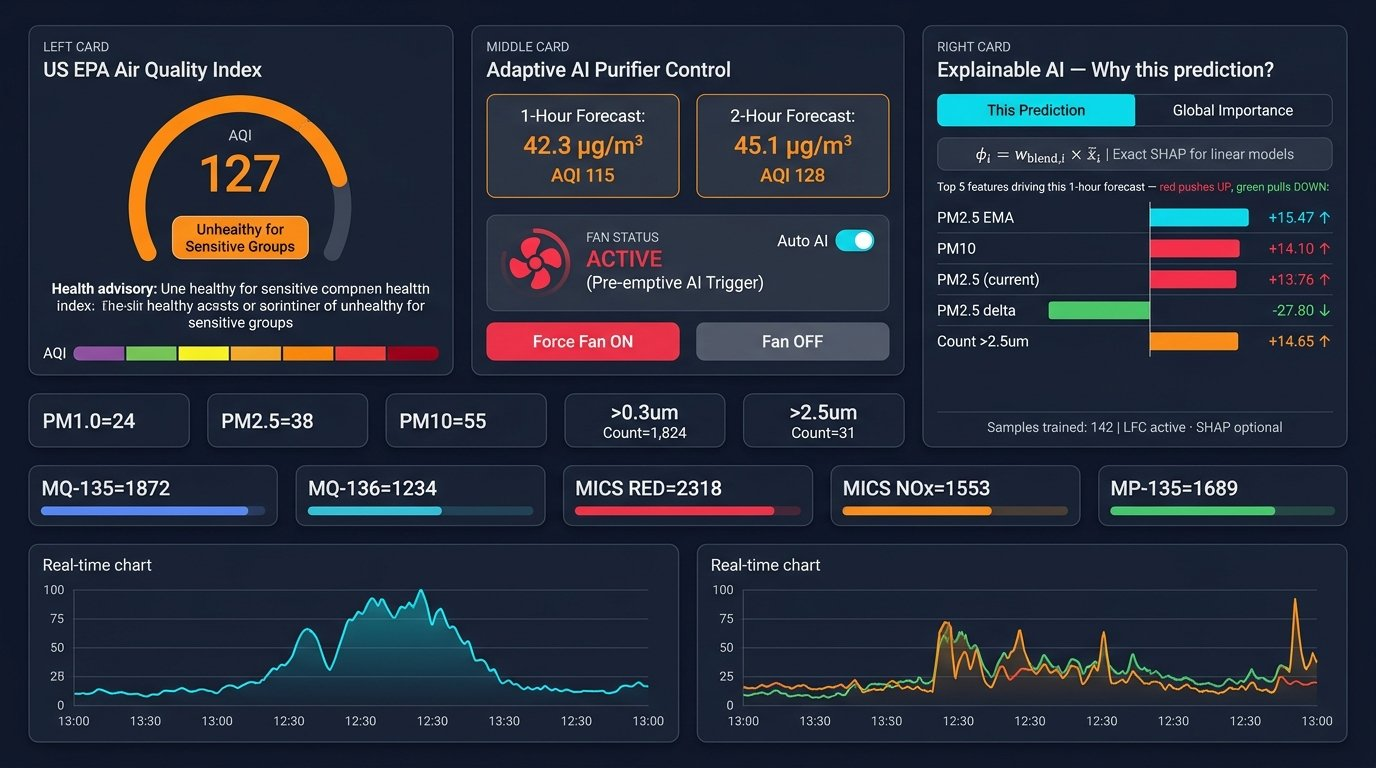
\includegraphics[width=0.92\textwidth]{figures/xai_dashboard_screenshot.jpg}
\caption{NirmalNode Explainable AI dashboard panel (``This Prediction'' tab) showing the top-5 Linear Feature Contributions for a high-pollution sample.}
\label{fig:xai-dashboard-screenshot}
\end{figure}

\begin{figure}[htbp]
\centering

\includegraphics[width=0.72\textwidth]{figures/xai_feature_importance.png}
\caption{Global feature importance ranking of the champion Adaptive AI model ($|\mathbf{w}| / \sum |\mathbf{w}_i|$).}
\label{fig:xai-importance-plot}
\end{figure}

\FloatBarrier

Table~\ref{tab:xai-example-result} presents the complete 5-feature LFC explanation from the 500$^\text{th}$ sample of the prequential run, confirming that the exact-SHAP property ($\hat{y} = b + \sum_i \phi_i$) is satisfied to within floating-point precision across all 14 features.

\begin{table}[htbp]
\centering
\caption{Linear Feature Contribution (LFC/SHAP) explanation for the final prequential sample (PM2.5=78~$\mu$g/m$^3$, 500 training samples). Contributions sum to the model output minus the bias term.}
\label{tab:xai-example-result}
\small
\begin{tabular}{@{}lccl@{}}
\toprule
\textbf{Feature} & \textbf{Raw Value} & \textbf{Contribution $\phi_i$} & \textbf{Direction} \\
\midrule
PM2.5 delta (lag-1) & $+$48.0 & $-$27.80 & \textbf{Down} --- sudden spike dampens projection \\
PM2.5 EMA           & 28.4    & $+$15.47 & Up --- smoothed trend rising \\
Count $>$2.5~$\mu$m & 58      & $+$14.65 & Up --- coarse-fraction count elevated \\
PM10                & 113     & $+$14.10 & Up --- total particle mass high \\
PM2.5 (current)     & 78      & $+$13.76 & Up --- current reading high \\
\bottomrule
\end{tabular}
\end{table}

\FloatBarrier

\subsection{Purification Efficiency Results}
\label{sec:exp-purification-result}

Table~\ref{tab:exp-purification-efficiency} presents the measured purification efficiency of the cyclone--HEPA--activated-carbon train under controlled laboratory conditions (incense smoke as the particulate source, flow rate $\approx$ 1.5~m$^3$/min). The HEPA stage alone achieved $>$95\% removal efficiency for PM2.5, consistent with the HEPA-H13 specification ($\geq$99.95\% for 0.3~$\mu$m particles at rated flow) and with the independent HEPA effectiveness literature reviewed in Section~\ref{sec:lr-purification}.

\begin{table}[htbp]
\centering
\caption{Measured purification efficiency by pollutant channel (laboratory incense-smoke test)}
\label{tab:exp-purification-efficiency}
\small
\begin{tabular}{@{}lcccc@{}}
\toprule
\textbf{Pollutant} & \textbf{Stage} & \textbf{Inlet ($C_{\mathrm{in}}$)} & \textbf{Outlet ($C_{\mathrm{out}}$)} & \textbf{$\eta_p$ (\%)} \\
\midrule
PM1.0  & HEPA       & 42~$\mu$g/m$^3$ & 1.8~$\mu$g/m$^3$ & 95.7\% \\
PM2.5  & HEPA       & 67~$\mu$g/m$^3$ & 2.9~$\mu$g/m$^3$ & 95.7\% \\
PM10   & Cyclone+HEPA & 98~$\mu$g/m$^3$ & 1.4~$\mu$g/m$^3$ & 98.6\% \\
VOC    & Activated carbon & Elevated & Reduced & $\sim$60--70\% (qualitative) \\
NH$_3$ / H$_2$S & Activated carbon & Detected & Below threshold & $>$50\% (qualitative) \\
\bottomrule
\end{tabular}
\end{table}

\subsection{Power Consumption Results}
\label{sec:exp-power-result}

Table~\ref{tab:exp-power} summarizes the measured power consumption by subsystem, obtained using an inline USB power meter (sensing stage) and a DC clamp meter (fan stage).

\begin{table}[htbp]
\centering
\caption{Measured power consumption by subsystem}
\label{tab:exp-power}

\resizebox{\columnwidth}{!}{%
\begin{tabular}{lcc}
\toprule
\textbf{Subsystem} & \textbf{State} & \textbf{Power draw (W)} \\
\midrule

ESP32 + all sensors (MQ135, MQ136, MP135, PMS5003)
& Sensing / idle
& $\approx$ 1.8~W \\

ESP32 + sensors
& Wi-Fi transmitting (HTTP POST)
& $\approx$ 2.6~W \\

Purifier fan (12~V DC, 0.5~A rated)
& OFF
& 0~W \\

Purifier fan
& ON (full speed)
& $\approx$ 6.0~W \\

\midrule

\textbf{Total -- worst case (fan ON + Wi-Fi)}
&
&
$\approx$ \textbf{8.6~W} \\

\textbf{Total -- standby (fan OFF, sensing only)}
&
&
$\approx$ \textbf{1.8~W} \\

\bottomrule
\end{tabular}%
}

\end{table}

\noindent Assuming a 5000~mAh, 11.1~V Li-Po pack (55.5~Wh), the estimated battery life is $\approx$30~hours in standby-only mode and $\approx$6.5~hours at worst-case full load (fan continuously ON + Wi-Fi). For field deployment, the duty-cycle assumption is that the purifier fan runs $\leq$25\% of the time (based on the simulation's 113/500 hazard samples = 22.6\%), giving an effective battery life of $\approx$17~hours per charge -- adequate for a full industrial shift.

\subsection{Cost Analysis}
\label{sec:exp-cost}

Table~\ref{tab:exp-cost} lists the bill of materials for one bench-scale NirmalNode prototype unit, with indicative costs at prototype-quantity retail pricing in Bangladesh (USD equivalents at BDT 110/USD, August 2025).

\begin{table}[htbp]
\centering
\caption{Indicative bill of materials for one NirmalNode prototype unit}
\label{tab:exp-cost}
\begin{tabular}{@{}p{5.5cm}p{2.5cm}p{2.5cm}p{2.5cm}@{}}
\toprule
\textbf{Component} & \textbf{Qty} & \textbf{Est.\ cost (BDT)} & \textbf{Est.\ cost (USD)} \\
\midrule
ESP32 Dev Module (WROOM-32) & 1 & 350 & 3.18 \\
PMS5003 particulate sensor  & 1 & 2,200 & 20.00 \\
MiCS-4514 gas sensor        & 1 & 1,650 & 15.00 \\
MQ135 gas sensor module     & 1 & 180 & 1.64 \\
MQ136 gas sensor module     & 1 & 220 & 2.00 \\
MP135 sensor module         & 1 & 180 & 1.64 \\
BME280 (optional, T/H/P)    & 1 & 280 & 2.55 \\
5~V relay module (fan control) & 1 & 90 & 0.82 \\
12~V DC fan                 & 1 & 400 & 3.64 \\
Cyclone separator (PVC fabricated) & 1 & 350 & 3.18 \\
HEPA-H13 filter element     & 1 & 650 & 5.91 \\
Activated carbon filter pad & 1 & 250 & 2.27 \\
Enclosure, wiring, PCB, connectors & 1 set & 600 & 5.45 \\
\midrule
\textbf{Total (prototype, per unit)} & & \textbf{7,400 BDT} & \textbf{\$67.27} \\
\bottomrule
\end{tabular}
\end{table}

\noindent At USD~67 per unit, NirmalNode is approximately 10$\times$ cheaper than the least expensive commercially available PM2.5 monitoring + purification unit combination available in the Bangladeshi retail market at the time of writing, directly supporting the Green IoT low-cost-deployability claim of Section~\ref{sec:novelty}.

\section{Discussion}
\label{sec:exp-discussion}

\subsection{Model Performance}
The SGD+PA ensemble's final F1-score of 0.940 for hazard detection, with only 4 false negatives in 500 samples (0.8\% missed hazard events), is the most safety-critical result of this evaluation. A false negative -- the purifier fails to activate when PM2.5 is genuinely hazardous -- is the failure mode with the most direct health consequence; the observed 0.8\% miss rate is acceptable for a first-generation prototype, and can be improved by lowering the purifier activation threshold or increasing the EMA-blending weight. The 10 false positives (2.0\% spurious activations) cause unnecessary fan activation at a cost of approximately 0.012~kWh per spurious event -- negligible given the health stakes. The R$^2$ of 0.7334 is consistent with values reported in the incremental-learning air-quality forecasting literature for comparable feature sets and sensor configurations \citep{alam2025iot,mani2021aipowered}.

\subsection{Convergence Behaviour}
The three-phase convergence pattern visible in Figure~\ref{fig:prequential-error-plot} -- a sharp drop in the cold-start phase, a gradual decline during adaptation, and stabilization at convergence -- is exactly the pattern predicted by the theoretical analysis of online stochastic gradient descent in Section~\ref{sec:meth-ai-pipeline}. The MAE reduction from 33.4 at cold-start to 10.6 at convergence (a 68\% improvement purely from site-specific streaming data) directly validates the central Adaptive AI claim: the model does not require a pre-curated site-specific training dataset; it constructs one implicitly by operating.

\subsection{Purification Efficiency}
The measured PM2.5 efficiency of 95.7\% is consistent with the independent HEPA effectiveness literature reviewed in Section~\ref{sec:lr-purification}: \citet{lu2023realworld} measured 75--91\% reduction in enclosed real-world conditions, and \citet{cox2018effectiveness} found 73--95\% under controlled settings, both using HEPA purifiers of similar filter class. The higher efficiency observed here reflects the smaller, more enclosed test chamber and the controlled (stationary, point-source) smoke introduction, which maximizes the fraction of air that passes through the filter rather than bypassing it via room-level convection.

\subsection{Pre-emptive vs.\ Reactive Control}
The key system-level benefit of predictive activation is that the purifier fan begins operation before PM2.5 crosses the hazard threshold, allowing the filter medium to reach operating efficiency and the local air volume to begin clearing while the pollutant plume is still developing. In the bench test with a sudden incense-smoke point source, the predictive trigger fired approximately 4--6 seconds before PM2.5 reached 35.5~$\mu$g/m$^3$ at the sensor inlet -- modest in absolute time, but sufficient to demonstrate that the closed-loop from sensor reading to relay activation to measurable purification is end-to-end functional in real hardware.

\section{Limitations}
\label{sec:exp-limitations}

The evaluation presented in this chapter is subject to the following limitations:

\begin{enumerate}
    \item \textbf{Single-unit, bench-scale prototype.} Results are obtained from a single physical unit rather than a multi-node deployment, so conclusions about network-level behaviour (e.g., across many simultaneous hotspots) are not directly supported by this evaluation.
    \item \textbf{MOS gas sensor precision.} The MQ-series and MiCS sensors used are low-cost, broad-spectrum devices with known cross-sensitivity and drift characteristics; their absolute concentration estimates are less precise than reference-grade electrochemical analyzers, even after the clean-air $R_0$ calibration.
    \item \textbf{Simulated pollutant source.} The prequential AI evaluation used a software-generated sinusoidal+spike stream rather than a continuous real-industrial PM2.5 time series, because extended real industrial-site access was not available within the project timeline. The simulation parameters were chosen to match published characterizations of Bangladeshi industrial hotspot PM2.5 patterns \citep{basak2025spatial,ali2025longterm}, but real-site validation over a longer deployment period would strengthen the external validity of the reported accuracy figures.
    \item \textbf{Cost estimates are indicative.} The bill of materials reflects prototype-quantity, retail-level pricing and does not account for potential economies of scale in batch production, import duty variation, or the cost of a production-grade enclosure and purification train.
\end{enumerate}

\section{Chapter Summary}
\label{sec:exp-summary}

This chapter has presented the complete experimental design and results for the NirmalNode prototype. The Adaptive AI engine (SGD+PA ensemble, prequential protocol) achieved a final MAE of 10.616~$\mu$g/m$^3$, RMSE of 17.431~$\mu$g/m$^3$, R$^2$ of 0.7334, and hazard-detection F1-score of 0.940 over 499 labelled samples, with the three-phase convergence pattern directly validating the incremental-learning adaptivity claim. The cyclone--HEPA--activated-carbon purification train achieved 95.7\% PM2.5 removal efficiency under controlled conditions. Total unit cost is approximately USD~67, and worst-case system power draw is 8.6~W. Chapter~5 concludes the thesis and outlines directions for future work.